\documentclass[]{spie}  %>>> use for US letter paper
%\documentclass[a4paper]{spie}  %>>> use this instead for A4 paper
%\documentclass[nocompress]{spie}  %>>> to avoid compression of citations

\renewcommand{\baselinestretch}{1.0} % Change to 1.65 for double spacing

\usepackage{amsmath,amsfonts,amssymb}
\usepackage{graphicx}
\usepackage[colorlinks=true, allcolors=blue]{hyperref}
\usepackage{subfigure}
\usepackage{float}
\usepackage{algorithm}
%\usepackage[options]{algorithm2e}
\usepackage[linesnumbered,lined,boxed,commentsnumbered,ruled]{algorithm2e}

\usepackage[noend]{algpseudocode}
\usepackage[redeflists]{IEEEtrantools}

\title{Priority coordination of fiber positioners\\
	in multi-objects spectrographs }

\author[a]{Dominique Tao}
\author[b]{Laleh Makarem}
\author[c]{Mohamed Bouri}
\author[d]{Jean-Paul Kneib}
\author[e]{Denis Gillet}
\affil[a,b,e]{REACT, Ecole Polytechnique Federale de Lausanne (EPFL), Switzerland}
\affil[c]{LSRO, Ecole Polytechnique Federale de Lausanne (EPFL), Switzerland}
\affil[d]{LASTRO, Ecole Polytechnique Federale de Lausanne (EPFL), Switzerland}

\authorinfo{Further author information:\\
	dominique.tao@alumni.epfl.ch, mohamed.bouri@epfl.ch, jean-paul.kneib@epfl.ch, denis.gillet@epfl.ch
}

% Option to view page numbers
\pagestyle{empty} % change to \pagestyle{plain} for page numbers   
\setcounter{page}{301} % Set start page numbering at e.g. 301

\begin{document} 
	\maketitle
	
	\begin{abstract}
		Projects such as "The Dark Energy Spectroscopic Instrument" (DESI)  [\citenum{2016arXiv161100037D}] or "The Multi Object Optical and Near-infrared Spectrograph" (MOONS ) [\citenum{8ad636d82d8a416f91dd848b1307de5f}] are developing spectrographs, composed of more than thousand of optical fibers in a confined hexagonal focal plane, to study the evolution of the universe. Such systems allow fast reconfiguration of the fibers as they are moved simultaneously to their assigned target by a 2-arm positioner within an short interval of time. Moreover, astronomers prioritize the observation of some objects over those that hold less information, creating a hierarchy of importances or priorities. In a scenario where not all the positioners can reach their targets, It is important to ensure the observation of the high-priority targets. \\
		In previous works, a decentralized navigation function from the family of potential fields was used for collision-free coordination. While it guarantees convergence of all the positioners to their targets for DESI [\citenum{MakaremDESIConference,makarem2015decentralized}], it fails at planning motion for positioners in MOONS [\citenum{MakaremMoons}]. The reason is that the second arm of the positioners in MOONS is two times the length of the first arm. Covering a larger working space, they are prone to deadlocks, a situation where two or more positioners are blocked by each other and so unable to reach their targets.\\
		In this paper and in the framework of MOONS project, we present our new approach to integrate assigned priorities with the decentralized navigation functions to reduce the deadlocks situations. For this purpose, we regulate the movements of the positioners using a finite-state machine combined with distance-based heuristics. Each positioner's state dictates its behaviors with respect to other positioners. Distance-based heuristics limit the states transition when a positioner is interacting with its adjacent positioners to localize possible deadlock situations. The advantage of this method is its simplicity as it relies on local interaction of positioners, keeping the complexity of the algorithm quasilinear. In addition, since it does not depend on the positioner's geometry, it is also scalable to other positioner kinematics. \\
		We developed a motion planning simulator with a graphic interface in python to validate the coordination of the positioners with assigned priorities.  As a result, the number of positioners converging to their targets improve from 60-70\% to 80-95\%. The computation time of the trajectories increases slightly due to the new layer of algorithm added for deadlocks prevention.
	\end{abstract}
	
	% Include a list of keywords after the abstract 
	\keywords{ MOONs, Optical fiber positioners, Priority coordination, Finite-state machine, distance-based heuristics}
	
	\section{INTRODUCTION}
	\label{INTRODUCTION}
	Recently uncovered that not only the universe is expanding but also that its process is accelerating, massive spectroscopic surveys are used in many international projects such as  "The Dark Energy Spectroscopic Instrument" (DESI) [\citenum{2016arXiv161100037D}] or  "The Multi Object Optical and Near-infrared Spectrograph" (MOONS) [\citenum{8ad636d82d8a416f91dd848b1307de5f}] to study its evolution. The used spectrographs are composed with more than thousand of optical fiber bundles, in a confined hexagonal focal plane. Each one are moving at the same time to a assigned target by a two arms robotics positioner, making real time observation possible.\\\\\\
	Anti-collision movement between positioners is therefore essential for a well-functioning system. While the completeness of the system, ie convergence of all positioners to their targets, is ensured with the project DESI using a decentralized navigation function algorithm  [\citenum{MakaremMoons,MakaremDESIConference,makarem2015decentralized}], the same approach is not valid for MOONS: its positioners second arm being two time longer as shown in figure ~\ref{MOONS_positioner_simulation} - ~\ref{DESI_positioner_representation}, it is covering a larger workspace and hence creating possible collisions and deadlocks, a situation where positioners, blocked by one another, are unable to reach their targets.\\
	
	\begin{figure}[H]
		\hspace{2cm}
		\begin{minipage}[t]{4.5cm}
			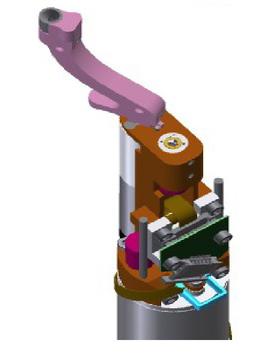
\includegraphics[scale=1.2]{images/realPositioner.jpg}
			\caption{CAD positioner model}
			\label{MOONS_positioner_representation}
		\end{minipage}
		\begin{minipage}[t]{5cm}
			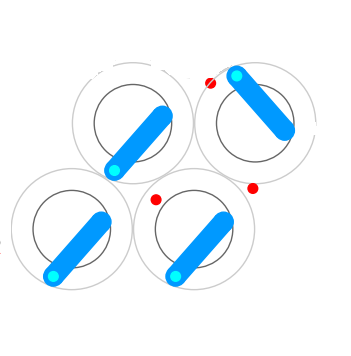
\includegraphics[scale=0.56]{images/MOONSPositioner_Simulation.png}
			\caption{MOONS positioner in simulation}
			\label{MOONS_positioner_simulation}
		\end{minipage}
		\begin{minipage}[t]{5cm}
			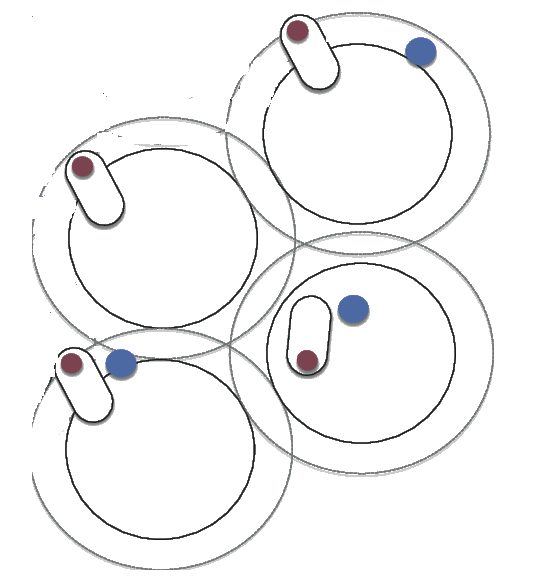
\includegraphics[scale=0.3]{images/DESI_Positioner.png}
			\caption{DESI positioner in simulation}
			\label{DESI_positioner_representation}
		\end{minipage}
	\end{figure}
			
	Though desirable, having a non complete system is not a serious issue since not all astronomical objects contain the same valuable information to study the universe evolution. Astronomers prefer to prioritize the observation of the important targets even at the price of disregarding the less relevant ones.\\\\
	With MOONS framework and as an extension of the previous work using a decentralized navigation function for collision avoidance [\citenum{MakaremMoons}], this paper explores an approach, through a finite state machine strategy, to take into account the importance/priority of each positioner's target into the coordination of their movements. As it gives more chance for higher priority positioners to reach their targets, its other objective is also to increase the positioners convergence with the goal of having a complete system.\\
		
	The organization of this paper is as followed: In section \ref{PRIORITY BASED COORDINATION}, a representation of the system and the finite state machine is described. Then we explain how deadlocks are localized and solved using an heuristic vector-distance based strategy. Section \ref{RESULTS} then presents the result of our approach on various test cases of positioner-configuration. As a conclusion, future research and possible improvements are discussed in section \ref{CONCLUSION}.
	
	\section{PRIORITY BASED COORDINATION}
	\label{PRIORITY BASED COORDINATION}
	
	
	Unlike many motion planning algorithms, the choice of using potential field to move simultaneously thousand of positioners stems from its computational simplicity. It enables fast computation of collision-free movements towards the targets of the positioners. However, due to local minimum problems, using simple potential field to handle more complex systems can exhibit deadlock situations. Therefore, benefiting from an algorithm based on potential fields requires either a more complex development of the algorithm or an additional layer of complexity.\\\\
	In this work, we design a decision layer using a finite state machine on top of a decentralized navigation function algorithm. Its role is to manage the interaction of positioners with different priorities. 

	\subsection{System representation}	
		\label{Finite-state machine} 
	
	 Figure \ref{MOONS_positioner_representation} - \ref{MOONS_positioner_simulation} - \ref{sys_representation} shows the MOONS positioner and its equivalent in simulation, where only the second arm (corresponding to the curve segment of the CAD model) is represented. The red dot is the target assigned to the positioner's end-effector, which holds the optic fiber represented by the dot at the extremity of the second arm.
		\begin{figure}[H]
			\centering
			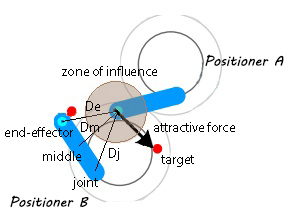
\includegraphics[scale=1]{images/system_representation.jpg}
			\caption{Representation of the variables in the system}
			\label{sys_representation}
		\end{figure}
	
	Let $p =$ \{$1,2,3,4$\} be the assigned priority to a positioner, with 4 for the most important target and 1 for the least important one. \\
	$D=$\{$D_e, D_m, D_j$\} is the set of distance between respectively the end-effector, middle and joint parts of one positioner to the  end-effector, middle or joint parts of another adjacent positioner. In figure \ref{sys_representation}, these distances are represented from positioner B to only the end-effector part of positioner A.\\\\
	As dictated by the principle of the potential field, each positioner is attracted to its target by a force $F_a$ and pushed away by the $i^{ieme}$ adjacent positioners with a repulsive forces, $F_{ri}$. Further details on their implementations in the context of MOONS are given in [\citenum{MakaremMoons}]. \\
	 With more than thousand positioners in a compact space and with each one having at most 6 neighbours, a "zone of influence", $Z_{F_{r}}$, is used for the repulsive forces. They are active only within this zone to limit and simplify the number of forces felt by one positioner from the others.\\ 
	 The zone $Z_{F_{r}}$ can be of any shape, but in this work, it was decided to be a circle around each part (end-effector, middle and joint) in order to have a simple cover on the whole positioner. The source of the repulsive force comes from the part of the neighbour positioner that is inside the zone $Z_{F_{r}}$.
	 
	\subsection{Finite-state machine}	
	
	The finite state machine has a total of 5 states with their corresponding transitions. Designed to take into account different priorities, it regulates the positioners interactions for a better coordination of the system.
	\subsubsection{First state: ON/OFF}
	\label{first_state_chap}
	The first state  is defined as the "ON/OFF" state. With the creation of a "ON/OFF zone", $Z_{ON/OFF}$, associated to a positioner, any neighbour positioners with a lower priority inside will have their attractive forces towards their targets disabled, ie $F_a = 0$. We refer to such a positioner as an OFF one in opposition to an ON one with its attractive force still active.
	Similarly to the influence zone $Z_{F_{r}}$, we use the same circle shape for $Z_{ON/OFF}$, centered on all parts of the positioner in order to entirely cover it.\\\\
	 With only repulsive forces to prevent collision, it allows the ON positioner with the higher priority to circulate through its OFF neighbours with less resistance, being the only one with an attractive force. This principle using priorities to solve the potential field local minima is illustrated in figure \ref{First_state}. 	
	\begin{figure}[H]
		\centering
		\begin{minipage}[t]{6.5cm}
			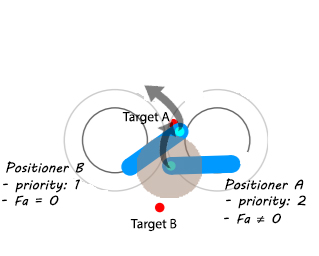
\includegraphics[scale=0.9]{images/first_state_0.jpg}
		\end{minipage}
		\begin{minipage}[t]{5cm}
			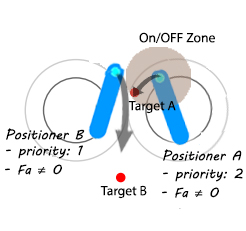
\includegraphics[scale=0.9]{images/first_state_ONOFF2.jpg}
		\end{minipage}
		\caption{\centering Principle of ON/OFF state (left to right image): \\
			(left image) Positioner B inside  $Z_{ON/OFF}$ of positioner A doesn't have any attractive force and is subject to repulsive force from positioner A, pushing it to the opposite direction of its target B. (right image) The same positioner B, once pushed out of the zone $Z_{ON/OFF}$  by positioner A, regains its attractive force.\\
\label{key}			}
		\label{First_state}
	\end{figure}
	
	A direct consequence of using only this state is the problem of deadlock due to oscillations between ON and OFF at the limit of the zone $Z_{ON/OFF}$. Considering an ON positioner A and its OFF neighbour B with lower priority inside the zone $Z_{ON/OFF}$ of A (figure \ref{First_state} right image), when the positioner B is at the border of the zone, it can be subject to the problem of reactivation and deac<tivation of its attractive force. If the reactivated attractive force is opposing the movement of the positioner A, it will re-enter the zone $Z_{ON/OFF}$ of A only to be repulsed again. This switching states can block the positioner A as the adjacent positioner B keeps oscillating at the same place.\\
	
	A deadlock can be interpreted when two or more adjacent positioners stop moving towards their targets because of each other, or oscillating indefinitely at the same place in space. A moving average filter on the positioner's velocity can be used to localize and unblock this situation by adding noise to it. Though it might be tempting to modify the magnitude of the different forces or of the noise, one has to consider the risk of collisions due to positioners sudden increase of velocity. \\
	Furthermore, only evaluating the velocity is necessary but not sufficient to detect a deadlock as explain later in the sub-chapter \ref{sub_chapter_fifth_state} since positioners can have a null velocity when arrived at their targets or when repulsing another one. \\\\
	With $v[t]$ the velocity of one positioner at time $t$, $y[t]$ is the output of the average moving filter of window $M$ such as:
	\begin{equation}
	\left\{
	\begin{IEEEeqnarraybox}[
	\IEEEeqnarraystrutmode
	\IEEEeqnarraystrutsizeadd{2pt}
	{2pt}
	][c]{rCl}
	y[t]& = & \dfrac{1}{M}\sum_{k=1}^{M}v[t-k]\\
	y[t] & < & thres \Rightarrow noise
	\end{IEEEeqnarraybox}
	\, \right.
	\label{}
	\end{equation} 
	We define $thres$ as the threshold representing the time the positioner is considered "stopped". The value of this constant is defined experimentally.
	The result $y[t]$ is used to introduce noise once it is under this threshold. 
		
	\subsubsection{Second \& third state: id and priority memorization}
	Having introduced new variables with the first state, we need to determine how positioners interact with each others depending not only on their assigned priority but also on their  ON and OFF states.\\\\
	Problematic situations can also occur with the interaction of more than two positioners. Similarly to the positioners configuration illustrated in figure \ref{ID_PR} (left image), deadlock can happen when two ON high priority positioners A and B are going against each other by propagating their opposite movements through an intermediate low priority OFF positioner C that is in-between them.\\\\
	To solve this problem, we use the principle of memorization by introducing two new states: 
	\begin{itemize}
		\item "MemPr":  \\
		Initialized at 0 for a positioner, it is used to memorize either the assigned priority or the MemPr of its neighbour positioner which has changed its  states.\\
		\item "MemId": \\
		Initialized at 0 for a positioner, it is used to memorize only the identity of its neighbour positioner which has changed its states.
	\end{itemize}\\
	  With this information and in a similar situation as in figure \ref{ID_PR}, one OFF positioner C, whose states has been changed by an ON neighbour positioner A due to its higher priority, is now able to change its other ON adjacent positioners states if their assigned priorities are smaller than the memorized priority "MemPr" of C. The positioner A, which changed the state of positioner C has its assigned priority memorized by C.  Put in another words, the positioner A is able, through C, to influence other non-adjacent positioners whose movements are opposing its one, allowing to have its convergence to its target A with less resistance.\\\\\\
	 We define this process as a "chain reaction": one OFF positioner can change the states of its neighbour positioner that is not the one that originally influenced it. \\
	 
	 To understand this principle and the assignments of values for "MemPr"  and "MemId", the pseudo-code of algorithm \ref{First_algo} gives a concise overview on how all the states seen so far for an considered positioner, called agent positioner, are changed when interacting with one of its neighbours. A visual step-by-step example following the algorithm \ref{First_algo} is illustrated in figure \ref{ID_PR}. \\\\
	 Furthermore, these rules are only valid if the agent positioner has not yet arrived to its target and is inside the $Z_{ON/OFF}$ zone of its neighbour positioner. This condition, represented by the line \ref{arr_condition_line}, involved the fourth state, "Arr", that is explained in the next sub-chapter \ref{sub_chap_fourth_state}. 
 	\begin{figure}[H]
 		\centering
 		\begin{minipage}[t]{5.2cm}

 			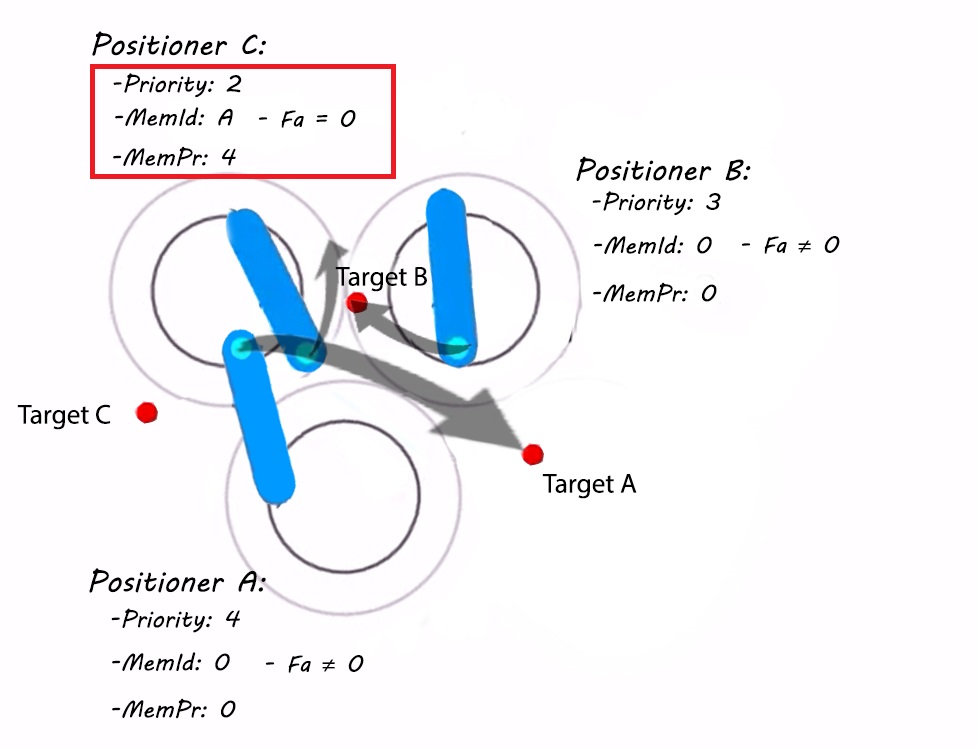
\includegraphics[scale=0.3]{images/ID_PR0.jpg}
 			\label{ID_PR0}
 		\end{minipage}
 		\begin{minipage}[t]{5.4cm}
 			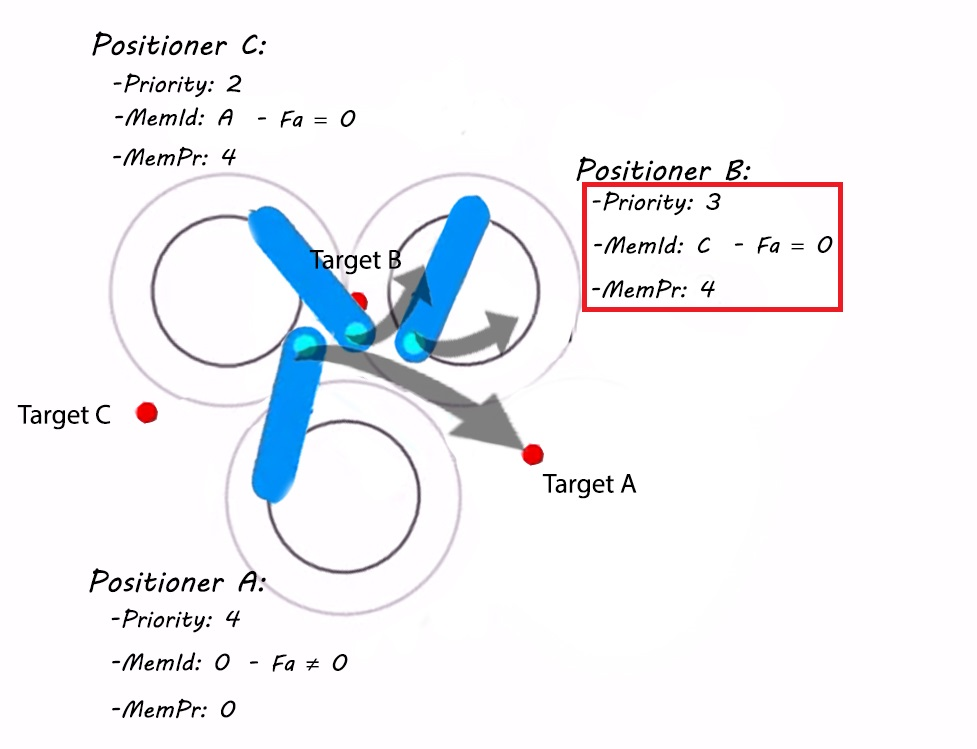
\includegraphics[scale=0.3]{images/ID_PR1.jpg}
 			\label{ID_PR1}
 		\end{minipage}
 		\begin{minipage}[t]{5.4cm}
 			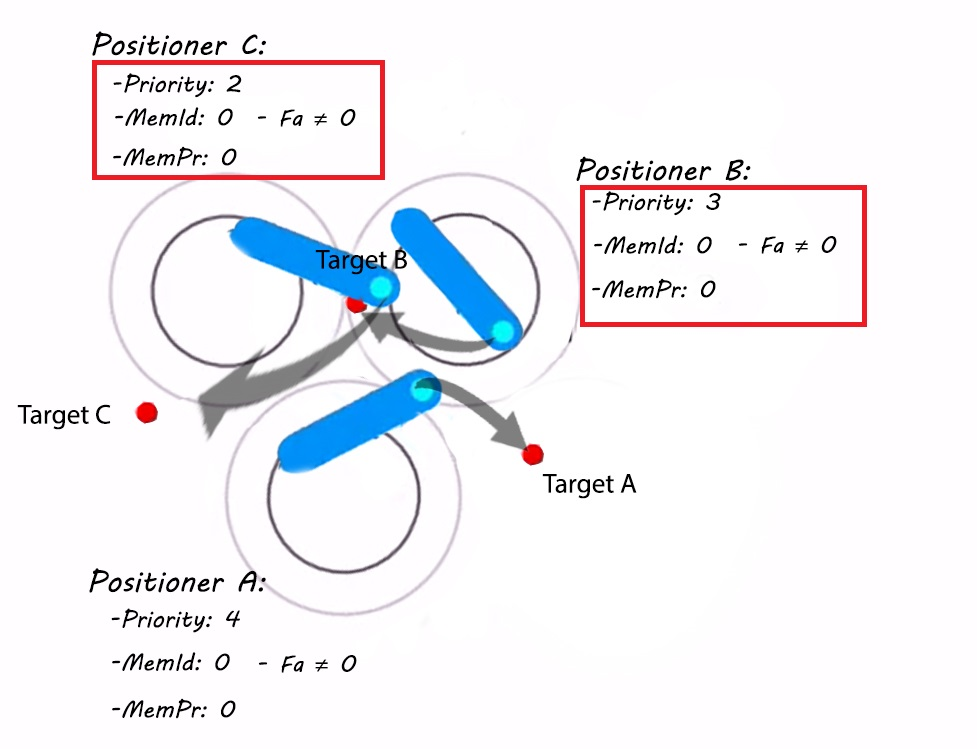
\includegraphics[scale=0.3]{images/ID_PR2.jpg}
 			\label{ID_PR2}
 		\end{minipage}
 		\caption{\centering Positioner chain reaction using MemId and MemPr states, obeying algorithm \ref{First_algo} for interaction:\\
 			(left image) Positioner A with the biggest priority influences its neighbour positioner C which remembers the priority and ID information of A when becoming OFF; (middle image) Even if positioner C assigned priority is smaller than the one from B, because C is OFF, B has to look on the memorized information of C: B having a smaller assigned priority, it becomes OFF and carry on the memorized priority of C; (right image) Once positioner A is out of the zone $Z_{ON/OFF}$ of C, deep first search algorithm using the memorized ID, "MemId" is used to recognize and reset all the states of all the positioners that entered the chain reaction process because of A }
 		\label{ID_PR}
 	\end{figure}
	   The four main conditions in lines \ref{condition1}, \ref{condition2}, \ref{condition3}, \ref{condition4}, in the algorithm \ref{First_algo} correspond to all the possible interactions of two adajacent positioners based on their ON/OFF states. It shows how the neighbour positioner states are compared with the agent ones and also how the values are assigned for the agent positioner states. Only the agent positioner states are modified. The reason is simply because algorithm \ref{First_algo} is applied to each positioner with respect to each of its adjacent positioners in the system.\\\\
	The general rule of comparison for the priorities in line \ref{comparison1}, \ref{comparison2}, \ref{comparison3}, \ref{comparison4} depends on the ON/OFF state of the positioner: if the positioner is ON, the assigned priority is used, otherwise the memorized priority, "MemPr". Then the values attributed to the "MemPr" state of the agent positioner follows the same logic.\\
	Therefore, all OFF positioners in the chain reaction remember the assigned priority of the only ON positioner, which is at the origin of this chain reaction.\\\\	
	In all cases, the agent positioner always remembers the ID of the neighbour positioner. It is used to track down all the positioners in the chain reaction.   
	\begin{algorithm}[H]
		\caption{agent\_status($agent$, $neighbour$)}\label{AlgoRedSoftEnve}
		\label{First_algo}
		\SetKwData{Left}{left}\SetKwData{This}{this}\SetKwData{Up}{up}
		\SetKwFunction{Union}{Union}\SetKwFunction{FindCompress}{FindCompress}
		\SetKwInOut{Input}{input}\SetKwInOut{Output}{output}
		\Output{For a considered positioner, called agent positioners, modification of its 1st, 2nd and 3rd states with respect to its considered neighbour positioner }
		
		\BlankLine
		\setcounter{AlgoLine}{0}
		\SetAlgoLined
		\uIf{agent.Arr == False  or neighbour == OFF \tcp*{"Arr" state introduced on sub-chapter \ref{sub_chap_fourth_state}}   \label{arr_condition_line} } 
		{		\BlankLine
			\uIf{agent == OFF and neighbour == OFF \label{condition1}}{
						\BlankLine
				\uIf{agent.MemPr $<$ neighbour.MemPr \label{comparison1}}{
					\BlankLine
					agent.MemId =  Neighbour Id\;\\
					agent.MemPr =  Neighbour.MemPr\;\\
				}
			}
			\uElseIf{agent == ON and neighbour == ON \label{condition2}}{
						\BlankLine
				\uIf{Agent Priority $<$ Neighbour Priority \label{comparison2}}{
					\BlankLine
					agent.ON/OFF = OFF \;\\
					agent.MemId =  Neighbour Id\;\\
					agent.MemPr =  Neighbour Priority\;\\
				}
			}
			\uElseIf{agent == OFF and neighbour == ON \label{condition3}}{
						\BlankLine
				\uIf{agent.MemPr $<$ Neighbour Priority \label{comparison3}}{
					\BlankLine
					agent.MemId =  Neighbour Id\;\\
					agent.MemPr =  Neighbour Priority\;\\
				}
			}
			\uElseIf{agent == ON and neighbour == OFF \label{condition4}}{
						\BlankLine
				\uIf{Agent Priority $<$ neighbour.MemPr \label{comparison4}}{
					\BlankLine
					 agent.ON/OFF = OFF \;\\
					agent.MemId =  Neighbour Id\;\\
					agent.MemPr =  Neighbour.MemPr\;
				}
			}
						\BlankLine
			\uIf{agent.MemId == Neighbour ID\label{conditionSame}}{
				\BlankLine
				Return indication Agent positioner states still being changed !
			}
	}
		\BlankLine
	\end{algorithm}
	 The lifetime of the memorization states, "MemId" and "MemPr", is bound to its agent positioner being OFF inside the $Z_{ON/OFF}$ zone of the neighbour positioner that has changed its states. Once outside, the states of the agent are re-initialized at their initial values, i.e. the first state at ON and the memorization states at 0. The states of all the other positioners that entered in the chain reaction process because of the agent positioner are also re-initialized. The algorithm of deep first search is used with the "MemId" information to recognize all the positioners in the chain reaction.\\\\
	When the algorithm \ref{First_algo} is reapplied again on the same two positioners, the agent positioner inside the $Z_{ON/OFF}$ zone of its neighbour positioner won't enter any of the conditions of the lines \ref{comparison1}, \ref{comparison2}, \ref{comparison3}, \ref{comparison4}  since its states were already changed previously by this same neighbour. The condition in line \ref{conditionSame} is added to ouptut that the agent positioner is still being affected by the same neighbour positioner, in order to avoid any complicated behaviors of the system.  

	
	\subsubsection{Fourth state: arrived}
	\label{sub_chap_fourth_state}
	With the assumption that a positioner A with the highest priority, $p = 4$, is already at destination, any lower priority positioners with their targets inside the zones $Z_{ON/OFF}$ and $Z_{F_{r}}$ of A are subject to repulsive forces and a change of their states. As a result the attractive forces of these lower priority positioners are disabled once inside the zones of A. They will be repulsed without resistance, and never reach their targets.\\
	\\
	This particular oscillation scenario is shown in figure \ref{fourth_state} with positioner A having a higher assigned priority than positioner B, whose target is inside the zones of A. Once inside the zone $Z_{ON/OFF}$ and $Z_{F_{r}}$, the positioner B changes to OFF and has its attractive force deactivated.
	\begin{figure}[H]
		\centering
		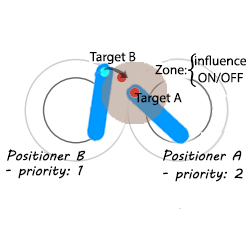
\includegraphics[scale=1]{images/fourth_state.jpg}
		\caption{\centering	Configuration of two positioners requiring the principle of the fourth state "Arr":\\
		Low-priority positioner B whose target B is inside a higher priority "already-arrived" positioner A zones $Z_{ON/OFF}$ and $Z_{F_{r}}$ }
		\label{fourth_state}
	\end{figure}
	In order to solve the problem of oscillation of the positioner near a high priority positioner, which has arrived to the target, we introduce a fourth state, "Arr". This state represents the positioner that has already arrived to its target. \\\\
	If a positioner A is in "Arr" state, it cannot change the states of any other positioner inside its zone $Z_{ON/OFF}$, regardless of their priorities. 
	Without having their attractive forces canceled, its neighbour positioners can converge to their targets that are inside the zone of A.\\\\
	In addition, the zone $Z_{F_{r}}$ of the already-arrived positioner has to be mitigated such that the repulsive forces felt by the neighbour positioners do not hinder their convergences, so we reduce the radius of the repulsion zone $Z_{F_{r}}$. Though two very close targets can make two positioners oscillate a little bit as the one arriving might repulse the one already arrived, both can stabilize and converge surprisingly well by adding some dead-zone between the end-effector and its target or time delay before the positioner exit its "Arr" state.  
	
	\subsubsection{Fifth state: deadlock and pseudo-priority}
	\label{sub_chapter_fifth_state}
	In order to have a clearer and better explanation of the fifth state, this sub-chapter is divided in three paragraphs: 
	\begin{enumerate}
		\item A description of the state and its principle 
		\item An explanation on how the states changes when interacting with other positioners
		\item Lastely, a method to detect situations which require the activation of the state
	\end{enumerate}
	
	\paragraph{State \& principle}\mbox{}\\
	So far, the finite state machine only regulates direct interactions between positioners with different priorities.
	When two positioners with the same priority but opposite movements directions enter in contact, deadlock situations are more probable to occur. A fifth and last state is added to the finite state machine to dictate the direct interaction between adjacent positioners with the same priorities.\\\\	
	To better understand the principle of this state, an analogy is done with an example of a well-known traffic problem, where two vehicles are being blocked by each other at one intersection. 
	In this kind of situation, the first goal of the drivers is not to reach their targets but to find a solution to the actual deadlock. In order to do that, they just "isolate" themselves from the rest to better determine which one should have the priority, as involving more vehicles into the deadlock will only make the problem more complicated to solve. To establish the best course of actions, each driver's evaluation is usually based on the indications of direction (the targeted direction) given by the other driver.\\
	
	With this example in mind, we define the fifth state, "lock\_sm". It is used to represent the positioner that is in a deadlock situation with another one that has the same priority value. For the rest of this paper, we refer to this specific situation as a "lock\_sm". \\\\
	Moreover, a pseudo-priority variable, "psPr", is associated to each positioner. It enables the system to obey the following principle, also illustrated in figure \ref{5thState}:\\
	When in a "lock\_sm" situation, the first goal of the two positioners B and C is not to reach their targets but to solve their current problem by determining which one should have the priority over the other. \\
	 To solve this situation more quickly, the distances from their end-effector to their respective targets are evaluated. The positioner with the smallest distance has a higher pseudo-priority. The pseudo-priority, "psPr" is only used for positioners in "lock\_sm" situation. All the interactions with the other positioners is regulated with the assigned or memorized priorities. \\\\
	To unblock a deadlock, the positioner B with higher pseudo-priority has an additional constant repulsive force from the target of the other positioner. The force can be formulated as a direct weighted relation with the average of the recent past velocities values of the positioner in order to diminish the risk of collision due to sudden speed increase.
	\begin{figure}[H]
		\centering
		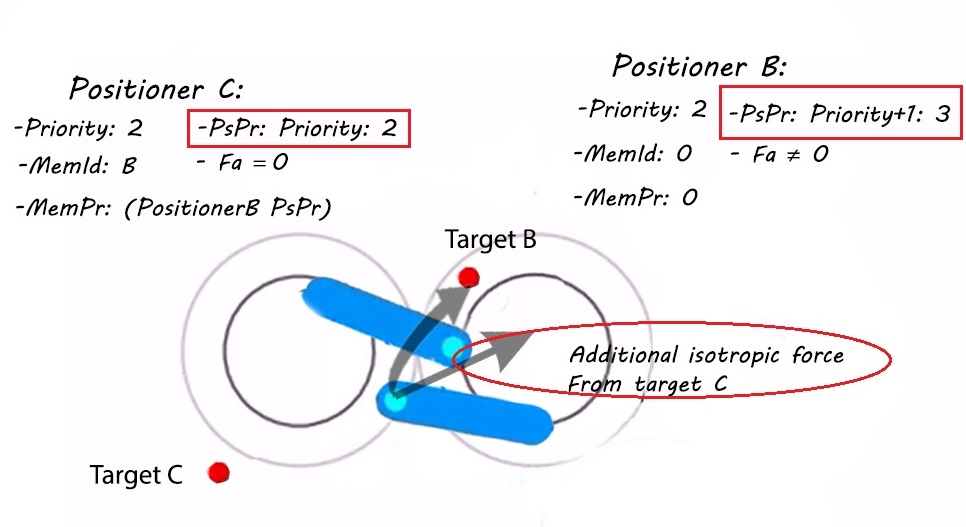
\includegraphics[scale=0.4]{images/5thstate.jpg}
		\caption{\centering Principle of 5th state, "lock\_sm", and pseudo-priority, "psPr" :\\
		With the same priority, inside their zone "$Z_{ON/OFF}$" and in "lock\_sm" situation, the distance from positioner B end-effector to its target is smaller compared to one from end-effector C to target C, the positioner B becomes more important symbolised by its pseudo-priority, "PsPr", being bigger and both fifth state being equaled to the ID of B}
		\label{5thState}
	\end{figure}
	\paragraph{Values \& interactions}\mbox{}\\
	The fifth state, "lock\_sm", and the pseudo-priority, "psPr", are both respectively initialized at 0 and at the assigned priority of the positioner. They are subject to a change of values when the considered positioner is inside the zone "$Z_{ON/OFF}$" of one of its neighbours and the configuration of this two adjacent positioners is considered leading to a "lock\_sm" situation. \\
	In case of a "lock\_sm" situation (figure \ref{5thState}), the pseudo-priority of the positioner deemed the most important one is increased by 1, while both positioner's fifth states "lock\_sm" are being equaled to the ID of the most important positioner. The reason is to give a unique identification so the two positioners can be recognized among their neighgours that they are both together in a "lock\_sm" situation.\\ 
	
 The values of all the states depend not only on the ON/OFF state but also on the new introduced variables: "lock\_sm" and "psPr". The pseudo-code of algorithm \ref{First_algo} is then completed with conditions to take into account all these new possible interactions between positioners. \\
The reasoning on how to integrate these new cases is explained and also shown with algorithm \ref{Second_algo} which represents only the condition of line \ref{condition3} of algorithm \ref{First_algo} with both the agent and neighbour positioners being OFF. The same logic is applied to complete the rest of the conditions in lines \ref{condition1}, \ref{condition2} and \ref{condition4} of algorithm \ref{First_algo}.\\\\
Because of the possible values of the fifth state, if it is bigger than 0, then the agent positioner is in a "lock\_sm" situation, not necessarily with the considered neighbour for the algorithm 1 which can also be in another "lock\_sm" situation with an other positioner. As a positioner can basically be either in a "lock\_sm" or not, four combinations for the fifth state are present as illustrated with the lines \ref{Alg2condition1}, \ref{Alg2condition2}, \ref{Alg2condition3} and \ref{Alg2condition4} of algorithm \ref{Second_algo}.\\
With a total of three priorities (assigned, memorized and pseusdo priority), their comparisons in the lines \ref{Alg2comparison1}, \ref{Alg2comparison2}, \ref{Alg2comparison3} and \ref{Alg2comparison4} of algorithm \ref{Second_algo}, and also in general for the system obey the following logic:\\
\begin{itemize}
\item If both positioners are not in a "lock\_sm" situation (line \ref{Alg2condition1}), their interactions follow the rules established in algorithm \ref{First_algo}.\\
\item If the positioners are both in a "lock\_sm" situation (line \ref{Alg2condition4}), the OFF positioner is still using its memorized priority "MemPr", but the pseudo-priority "PsPr" is used instead of the assigned priority for the ON positioner. Consequently, the agent positioner memorizes the pseudo-priority of its neighbour.\\
\item If one positioner is in a "lock\_sm" situation and the other is not, as shown in lines \ref{Alg2condition2} and \ref{Alg2condition3}, one has to think back with the example of the traffic jam problem where two vehicles are blocked at an intersection. As mentioned, involving more vehicles into the deadlock situation is unwanted, which is why the pseudo-priority is not used at all for this mix-cases.
\begin{itemize}
\item If the two positioners are ON, then both use their assigned priorities.\\
\item If the two positioners are OFF, the one that is in a "lock\_sm" situation uses its assigned priority while the memorized priority "MemPr" is used by the other.\\  
\item For their ON/OFF mixed cases, we can push forward the reasoning with the vehicles problem to understand the reason of the priority comparison.\\ 
If we consider the two vehicles in the deadlock situation to be the most important one (a deadlock with two ambulances), then an external less important one (a tourist vehicle) won't be able to influence them. As a matter of fact, even if one ambulance becomes less important than the other one in order to solve the deadlock, it is still an ambulance that cannot be less important than a simple tourist vehicle.\\
Following this logic, a positioner that is in a "lock\_sm" situation, regardless of being ON or OFF, still uses its assigned priority. The other positioner not involved in the deadlock uses either its "MemPr" if OFF, or its assigned priority if ON. 

\end{itemize}
\end{itemize}	
For any combination of their ON/OFF states, when the agent positioner in a "lock\_sm" situation has been influenced by its neighbour that is not in a "lock\_sm" situation, it means that the neighbour was able to break out the deadlock situation because of its higher importance. Consequently, both the agent and the neighbour positioner together in the "lock\_sm" situation have their fifth states and pseudo-priorities re-initialized.\\
The agent positioner always memorizes the priority that the neighbour positioner uses for the priority comparison. Similarly, the agent always memorizes the Id of the neighbour (not its MemId). 
		\begin{algorithm}[H]
			\caption{Completion of the condition in line \ref{condition3} in algorithm \ref{First_algo}}
			\label{Second_algo}
			
			 \KwData{All possible interactions between a considered OFF positioner, called agent positioner, and its ON neighour}
\setcounter{AlgoLine}{0}
		\SetAlgoLined
		\uIf{agent == OFF and neighbour == ON    \label{Alg2condition_line} } 
		{		\BlankLine
			\uIf{agent.lock\_sm $>$ 0 and neighbour.lock\_sm $>$ 0 \label{Alg2condition1}}{
						\BlankLine
				\uIf{agent.MemPr $<$ neighbour.PsPr \label{Alg2comparison1}}{
					\BlankLine
					agent.MemId =  Neighbour Id\;\\
					agent.MemPr =  Neighbour.PsPr\;\\
				}
			}
			\uElseIf{agent.lock\_sm $>$ 0 and  neighbour.lock\_sm == 0 \label{Alg2condition2}}{
						\BlankLine
				\uIf{Agent Priority $<$ Neighbour Priority \label{Alg2comparison2}}{
					\BlankLine
					
					Reset\_Both\_Positioners\_FifthState()\\
					Reset\_Both\_Positioners\_PseudoPriority()\\
					agent.MemId =  Neighbour Id\;\\
					agent.MemPr =  Neighbour Priority\;\\
				}
			}
			\uElseIf{agent.lock\_sm == 0 and  neighbour.lock\_sm $>$ 0 \label{Alg2condition3}}{
						\BlankLine
				\uIf{agent.MemPr $<$ Neighbour Priority \label{Alg2comparison3}}{
					\BlankLine
					agent.MemId =  Neighbour Id\;\\
					agent.MemPr =  Neighbour Priority\;\\
				}
			}
			\uElseIf{agent.lock\_sm == 0 and  neighbour.lock\_sm == 0 \label{Alg2condition4}}{
						\BlankLine
				\uIf{agent.MemPr $<$ Neighbour Priority \label{Alg2comparison4}}{
					\BlankLine
					agent.MemId =  Neighbour Id\;\\
					agent.MemPr =  Neighbour Priority\;
				}
			}
			}
			\BlankLine
		\end{algorithm}
	
	\paragraph{Deadlock "lock\_sm" localization}\mbox{}\\
	In this paragraph, the objective is to describe how we consider the configuration between two positioners to be a "lock\_sm" situation.\\
	With two adjacent positioners, called agent positioner and its neighbour, having an equal assigned priority and being inside their zones "$Z_{ON/OFF}$", we use the "point of view" from both their closest parts (end-effector, middle or joint) to assess the possibility of deadlock.\\
	The "point of view" can be understood as how the agent is seeing its target and its neighbours target with respect to its neighbour positioner closest part.
	Mathematically, as illustrated in figure \ref{projection},  we define it as the projection of the agent and neighbour targets on a line created by the vector between the closest parts of both positioners.\\
	\begin{figure}[H]
		\centering
		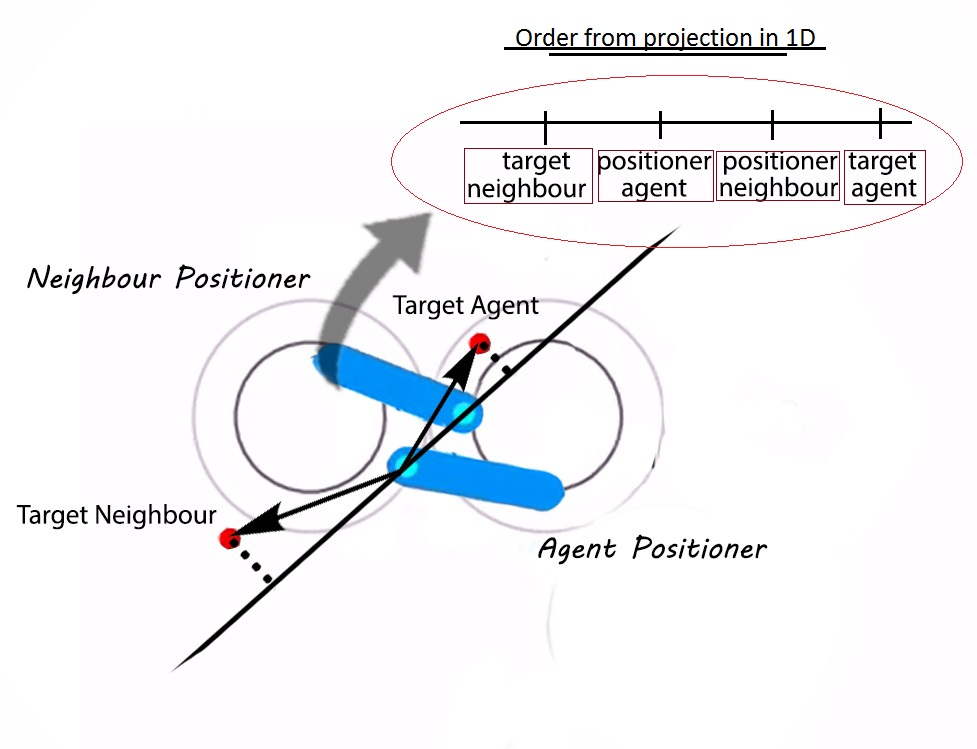
\includegraphics[scale=0.35]{images/Projection1.jpg}
		\caption{\centering Point of view in 1D configuration:\\
			 Projection of agent and neighbour targets on the line created from closest parts (end-effector, middle or joint) of both positioners}
		\label{projection}
	\end{figure}
	It basically projects everything into a line in order to evaluate in 1D if the agent target is on the same side as the agent positioner or is behind the neighbour positioner. For the latter case as shown in figure \ref{projection}, the neighbour positioner becomes an obstacle to the movement of the agent one, possibly leading to a deadlock situation. We then compare the projection with a look-up table that contains all possible 1D configurations of the agent, neighbour positioners and their targets placed in 1 line (24 possible permutations).\\
	The logic to distinguish which 1D configuration is considered a deadlock is simply to individually assess for each configuration if there is any collision with both positioners movements towards their targets on the 1D line. The example in figure \ref{look_UpTableLogic} shows the reasoning with few examples which can be generalized to determine the nature for rest of the 1D configurations.\\\\
		Since the movement of the positioner is planar with 2 degree of freedom, having the point of view from both agent and neighbour positioners allows a better perspective of the current configuration. As such, the consequence is that if their configuration is considered as a deadlock from the point of view of one positioner, then both positioners are in deadlock situation. In other words, we only need one projections to be a 1D configuration deadlock in order to consider the whole situation as a "lock\_sm" one. 	
	\begin{figure}[H]
		\centering
		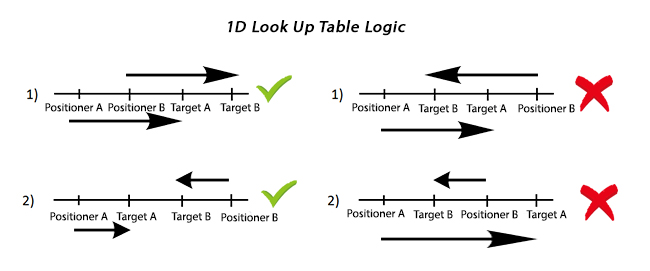
\includegraphics[scale=0.50]{images/1DLookUpTable.jpg}
		\caption{\centering
			 Configuration examples of look up table logic:\\
			On the left column, positioner A and B movements are hindering each other; 
			On the right column,  the positioner B ending up at its target  hinders the movement of positioner A to its target, being in between them. }
		\label{look_UpTableLogic}
	\end{figure}\\ 
	\section{Simulation \& RESULTS}
	\label{RESULTS}
	\subsection{Software \& hardware}
	\label{Software Hardware}
	To evaluate our approach, a simulator developed in python which recreates the shape and the behavior of the positioners is used. The trajectories of the positioners are first pre-computed and then directly given in open-loop to the electronics controlling the motors.\\  
	All simulation tests were conducted on a Lenovo thinkpad T450s with an Intel Core i7-5600U @ 2.69GHz x 4 processor, GeForce 940M SSE2 graphic card on an ubuntu 14.04 LTS version.
	\subsection{Tests \& results}
	\label{Test cases}
	
	Repeatability tests are done in order to assess the performance and efficiency of our approach. For this purpose, we compare the results obtained from our finite state machine (FSM) with the ones using only the decentralized navigation function algorithm (Without FSM). In the latter case, the assigned priorities are not taken into account as there are no mechanism to do so.\\\\
	In addition to all the figures seen so far which are real working examples of positioners interactions with different priorities, the goal is also to assess the robustness of the algorithm to coordinate a whole system of positioners with a hierarchy of importance.
	
	\subsubsection{Repeatability: convergence and time performance}
	We run our algorithm on 8 different test files. Each represents one specific and unique initial configuration of thousand of positioners with their respective targets. All positioners have the same assigned priority value.\\\\
	Each configuration file is used to evaluate the following performances: 
	\begin{itemize}
		\item Number of positioners successfully converging to their targets.
		\item Time in seconds necessary for the pre-computation of their movements.
	\end{itemize}
	The goal is not only to verify if the performance of our algorithm is repeatable over different configurations of our system but also if it is acceptable to use it in real time.\\
	To this end, for each configuration test file, the total number of around a thousand of positioners is partitioned into 12 subsets of sub-total positioners, on which we run our algorithm. The results are given in figures \ref{configuration1_result}, \ref{configuration2_result}, \ref{configuration3_result}, \ref{configuration4_result}, \ref{configuration5_result}, \ref{configuration6_result}, \ref{configuration7_result}, \ref{configuration8_result}.
	
	\begin{figure}[H]
		\begin{minipage}{8.7cm}
			\begin{minipage}[t]{4.3cm}
				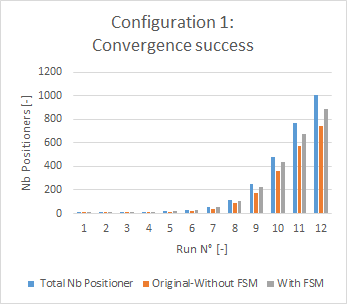
\includegraphics[scale=0.56]{images/configuration1_conv}
				\label{configuration1_conv}
			\end{minipage}
			\begin{minipage}[t]{1.0cm}
				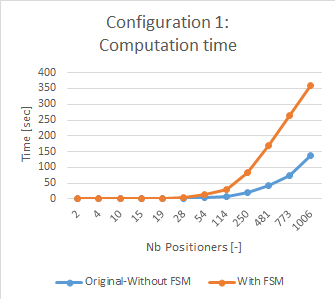
\includegraphics[scale=0.57]{images/configuration1_time}
				\label{configuration1_time}
			\end{minipage}
			\caption{\centering Configuration 1:\\
				 Convergence success and computation time data
				 \begin{itemize}
	 					 	\item With FSM: Decentralized navigation function with finite state machine
	 					 	\item Without FSM: Decentralized navigation function without finite state machine
				 \end{itemize}
			\tiny
			\begin{tabular}{|l|l|l|l|l|l|l|l|}
					\hline
					\multicolumn{2}{|l|}{Total Positioners}  & 54 & 114 & 250 & 481 & 773 & 1006\\
					\hline
					Conv. & With FSM  & 52 & 105  & 228 & 434 & 675 & 889 \\
					\cline{2-8}
						 & Without FSM & 41  & 88 & 176 & 358 & 577 & 747 \\
					\hline
					Time\\(sec) & With FSM  & 13.8 & 30.9  & 84 & 169.7 & 265.2 & 360.1 \\
					\cline{2-8}
					& Without FSM  & 3.5  & 8.6 & 21.4 & 43.7 & 74.5  & 136.1 \\
					\hline
			\end{tabular}}
				\label{configuration1_result}
		\end{minipage}
		\begin{minipage}{9cm}
			\begin{minipage}[t]{4.2cm}
				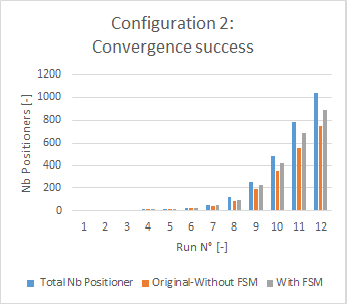
\includegraphics[scale=0.56]{images/configuration2_conv}
				\label{configuration1_conv}
			\end{minipage}
			\begin{minipage}[t]{1.0cm}
				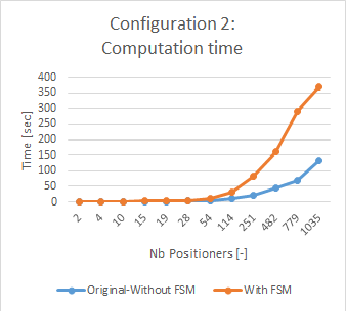
\includegraphics[scale=0.56]{images/configuration2_time}
				\label{configuration1_time}
			\end{minipage}
			\caption{\centering Configuration 2:\\
				Convergence success and computation time data
				 \begin{itemize}
							 	\item With FSM: Decentralized navigation function with finite state machine
							 	\item Without FSM: Decentralized navigation function without finite state machine
				 \end{itemize}
							\tiny
				\begin{tabular}{|l|l|l|l|l|l|l|l|}
					\hline
					\multicolumn{2}{|l|}{Total Positioners}  & 54 & 114 & 251 & 482 & 779 & 1035\\
					\hline
					Conv. & With FSM  & 52 & 103  & 231 & 415 & 679 & 892 \\
					\cline{2-8}
					& Without FSM & 45  & 91 & 189 & 350 & 555 & 750 \\
					\hline
					Time\\(sec) & With FSM  & 11.8 & 31  & 81.2 & 159.2 & 291.7 & 369.7 \\
					\cline{2-8}
					& Without FSM  & 3.8  & 9.6 & 21.6 & 44 & 69.9  & 134.1 \\
					\hline
				\end{tabular}
				}
			\label{configuration2_result}
			\end{minipage}
	\end{figure}
\begin{figure}[H]
	\begin{minipage}{8.7cm}
		\begin{minipage}[t]{4.3cm}
			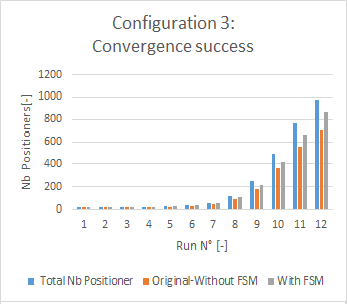
\includegraphics[scale=0.56]{images/configuration3_conv}
			\label{configuration1_conv}
		\end{minipage}
		\begin{minipage}[t]{1.0cm}
			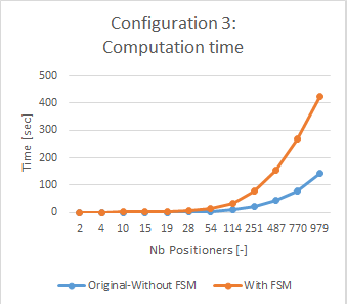
\includegraphics[scale=0.57]{images/configuration3_time}
			\label{configuration1_time}
		\end{minipage}
		\caption{\centering Configuration 3:\\
			Convergence success and computation time data
			\tiny
			\begin{tabular}{|l|l|l|l|l|l|l|l|}
				\hline
				\multicolumn{2}{|l|}{Total Positioners}  & 54 & 114 & 251 & 487 & 770 & 979\\
				\hline
				Conv. & With FSM  & 53 & 101  & 217 & 413 & 665 & 864 \\
				\cline{2-8}
				& Without FSM & 41  & 86 & 181 & 358 & 554 & 704 \\
				\hline
				Time\\(sec) & With FSM  & 14 & 32.3  & 79.9 & 155.1 & 267.2 & 425.2 \\
				\cline{2-8}
				& Without FSM  & 3.7  & 9.1 & 21 & 45.2 & 79.2  & 143.6 \\
				\hline
			\end{tabular}
			}
			\label{configuration3_result} 
		\end{minipage}
		\begin{minipage}{9cm}
			\begin{minipage}[t]{4.2cm}
				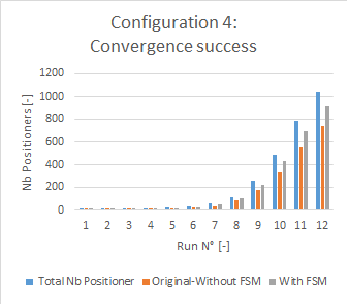
\includegraphics[scale=0.56]{images/configuration4_conv}
				\label{configuration1_conv}
			\end{minipage}
			\begin{minipage}[t]{1.0cm}
				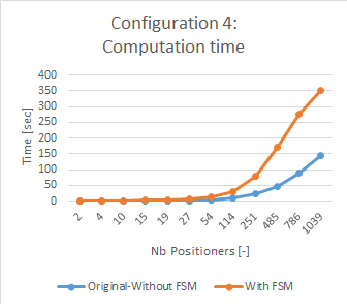
\includegraphics[scale=0.56]{images/configuration4_time}
				\label{configuration1_time}
			\end{minipage}
			\caption{\centering Configuration 4:\\
				Convergence success and computation time data
				\tiny
				\begin{tabular}{|l|l|l|l|l|l|l|l|}
					\hline
					\multicolumn{2}{|l|}{Total Positioners}  & 54 & 114 & 251 & 485 & 786 & 1039\\
					\hline
					Conv. & With FSM  & 48 & 103  & 222 & 436 & 698 & 914 \\
					\cline{2-8}
					& Without FSM & 35  & 81 & 172 & 339 & 553 & 742 \\
					\hline
					Time\\(sec) & With FSM  & 13.4 & 30.8 & 79.6 & 170.4 & 274.1 & 352.1 \\
					\cline{2-8}
					& Without FSM  & 3.8  & 9.3 & 23.9 & 47.3 & 89.5  & 144.9 \\
					\hline
				\end{tabular}
				}
				\label{configuration4_result} 
			\end{minipage}
		\end{figure}
\begin{figure}[H]
	\begin{minipage}{8.7cm}
		\begin{minipage}[t]{4.3cm}
			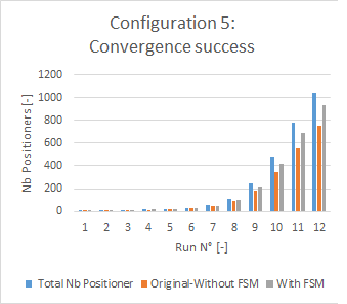
\includegraphics[scale=0.56]{images/configuration5_conv}
			\label{configuration1_conv}
		\end{minipage}
		\begin{minipage}[t]{1.0cm}
			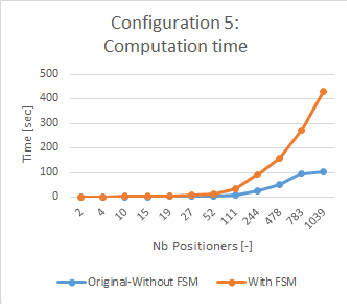
\includegraphics[scale=0.57]{images/configuration5_time}
			\label{configuration1_time}
		\end{minipage}
		\caption{\centering Configuration 5:\\
			Convergence success and computation time data
			\tiny
			\begin{tabular}{|l|l|l|l|l|l|l|l|}
				\hline
				\multicolumn{2}{|l|}{Total Positioners}  & 52 & 111 & 244 & 478 & 783 & 1039\\
				\hline
				Conv. & With FSM  & 50 & 105  & 219 & 421 & 689 & 931 \\
				\cline{2-8}
				& Without FSM & 44  & 89 & 186 & 349 & 555 & 754 \\
				\hline
				Time\\(sec) & With FSM  & 12.9 & 32.7  & 91.8 & 155.9 & 267.8 & 429.7 \\
				\cline{2-8}
				& Without FSM  & 3.8  & 8.7 & 24.1 & 47.2 & 93.3  & 103.4 \\
				\hline
			\end{tabular}
			}
			\label{configuration5_result} 
		\end{minipage}
		\begin{minipage}{9cm}
			\begin{minipage}[t]{4.2cm}
				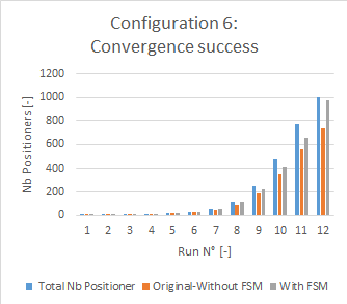
\includegraphics[scale=0.56]{images/configuration6_conv}
				\label{configuration1_conv}
			\end{minipage}
			\begin{minipage}[t]{1.0cm}
				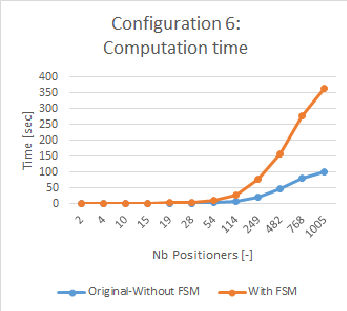
\includegraphics[scale=0.56]{images/configuration6_time}
				\label{configuration1_time}
			\end{minipage}
			\caption{\centering Configuration 6:\\
				Convergence success and computation time data
				\tiny
				\begin{tabular}{|l|l|l|l|l|l|l|l|}
					\hline
					\multicolumn{2}{|l|}{Total Positioners}  & 54 & 114 & 249 & 482 & 768 & 1005\\
					\hline
					Conv. & With FSM  & 54 & 110 & 225 & 415 & 651 & 973 \\
					\cline{2-8}
					& Without FSM & 47  & 90 & 187 & 356 & 561 & 734 \\
					\hline
					Time\\(sec) & With FSM  & 12 & 28.8 & 76.3 & 158.6 & 275.9 & 364.2 \\
					\cline{2-8}
					& Without FSM  & 3.9  & 8.6 & 22.6 & 46.4 & 79.8  & 101.2 \\
					\hline
				\end{tabular}
				}
				\label{configuration6_result} 
			\end{minipage}
		\end{figure}
\begin{figure}[H]
	\begin{minipage}{8.7cm}
		\begin{minipage}[t]{4.3cm}
			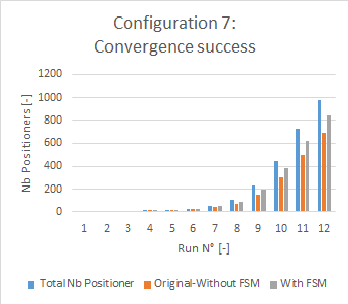
\includegraphics[scale=0.56]{images/configuration7_conv}
			\label{configuration1_conv}
		\end{minipage}
		\begin{minipage}[t]{1.0cm}
			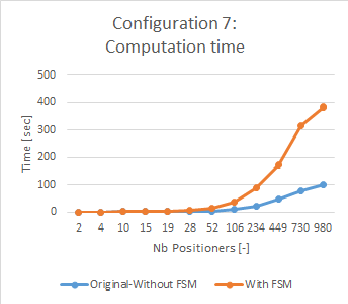
\includegraphics[scale=0.57]{images/configuration7_time}
			\label{configuration1_time}
		\end{minipage}
		\caption{\centering Configuration 7:\\
			Convergence success and computation time data
			\tiny
			\begin{tabular}{|l|l|l|l|l|l|l|l|}
				\hline
				\multicolumn{2}{|l|}{Total Positioners}  & 52 & 106 & 234 & 449 & 730 & 980\\
				\hline
				Conv. & With FSM  & 50 & 90  & 196 & 382 & 621 & 844 \\
				\cline{2-8}
				& Without FSM & 40  & 72 & 155 & 300 & 503 & 691 \\
				\hline
				Time\\(sec) & With FSM  & 14.4 & 36.2  & 89 & 172.8 & 315.8 & 383 \\
				\cline{2-8}
				& Without FSM  & 3.9  & 8.6 & 21.1 & 46.8 & 76.5  & 102.1 \\
				\hline
			\end{tabular}
			}
		\label{configuration7_result} 
		\end{minipage}
		\begin{minipage}{9cm}
			\begin{minipage}[t]{4.2cm}
				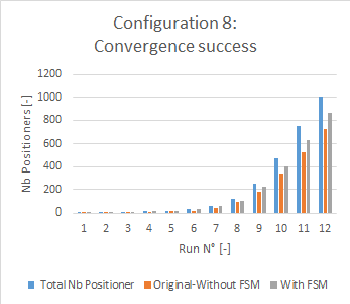
\includegraphics[scale=0.56]{images/configuration8_conv}
				\label{configuration1_conv}
			\end{minipage}
			\begin{minipage}[t]{1.0cm}
				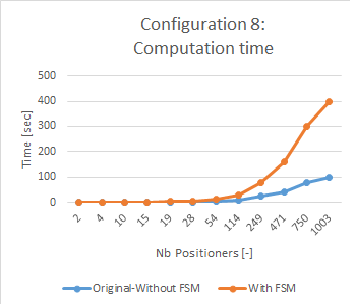
\includegraphics[scale=0.56]{images/configuration8_time}
				\label{configuration1_time}
			\end{minipage}
			\caption{\centering Configuration 8:\\
				Convergence success and computation time data
				\tiny
				\begin{tabular}{|l|l|l|l|l|l|l|l|}
					\hline
					\multicolumn{2}{|l|}{Total Positioners}  & 54 & 114 & 249 & 471 & 750 & 1003\\
					\hline
					Conv. & With FSM  & 52 & 103 & 221 & 401 & 630 & 861 \\
					\cline{2-8}
					& Without FSM & 40  & 86 & 179 & 342 & 525 & 723 \\
					\hline
					Time\\(sec) & With FSM  & 12.3 & 29.2 & 78.2 & 161.9 & 301.2 & 399.5 \\
					\cline{2-8}
					& Without FSM  & 4  & 9.2 & 23.0 & 42.7 & 78.3  & 99.5 \\
					\hline
				\end{tabular}}
				\label{configuration8_result} 
			\end{minipage}
		\end{figure}					
	For all the configuration tests, the general evolution of the results remains similar: when using the finite state machine, we can observe an improvement of positioners convergence from 60-70\% to 80-95\%.\\
	The computation time increases almost linearly. It is an expected result since we added another layer of computation to the already existing algorithm that we use for comparison. With better optimization such as parallel computation and/or more performant hardwares, a better time performance can be achieved.\\\\
	 Although positioners have the same priorities in our simulations, the improvement in convergence demonstrates the robustness of our algorithm to take into account different priorities. Due to the mechanism of the fifth state of the finite state machine, interactions of positioners with similar priorities also involve all the other states as their priorities become locally different. 	
	\section{CONCLUSION}
	\label{CONCLUSION}
	In the context of the MOONS project and as an extension of [\citenum{MakaremMoons}], an approach with a finite state machine is built on top of a decentralized navigation function from the potential field family. It enables better coordination of a multi-objects positioners inside a hexagonal confined space. With its different states, it takes into account different priorities assigned to each positioner, creating a hierarchy of importance where positioners with higher priority have more probabilities to reach their targets. Along with the possibility to manage deadlocks, it enables a better convergence of the system:
	 an improvement from  60-70\% to 80-95\% of positioners in the system converging to their targets is observed from repeatability tests. The results are obtained from comparing our approach with the one using only the decentralized navigation function. Furthermore, the algorithm is scalable to other system configuration than MOONS as it doesn't depend on the positioner's geometry.\\
	Since we added another layer of complexity to an already existing algorithm, the trajectories computation time becomes slower, but kept in a  quasilinear order. One possible work can be to further optimize the algorithm by using the right optimization method such as parallel computing or more performant hardwares. Moreover, since our approach has no proof of completeness, more research on the algorithm for a better positioner convergence can be consider.
	Extending this approach to take into account other features, such as for the project SLOAN-SDSS5 that needs to select which (UV, visible or IR) optical fibers to use within one positioner is also a possibility. It is a subject which is particularly interesting for astronomers since not all objects in the universe can be well observed in the same range of the optic spectrum.
	
	\acknowledgments % equivalent to \section*{ACKNOWLEDGMENTS}       
	
	The authors would like to thank Ezequiel Gonzalez Debada for the brainstorming sessions.

% References
\bibliography{report} % bibliography data in report.bib
\bibliographystyle{spiebib} % makes bibtex use spiebib.bst

\end{document} 
